%%%%%%%%%%%%%%%%%%%%%%% file template.tex %%%%%%%%%%%%%%%%%%%%%%%%%
%
% This is a general template file for the LaTeX package SVJour3
% for Springer journals.          Springer Heidelberg 2010/09/16
%
% Copy it to a new file with a new name and use it as the basis
% for your article. Delete % signs as needed.
%
% This template includes a few options for different layouts and
% content for various journals. Please consult a previous issue of
% your journal as needed.
%
%%%%%%%%%%%%%%%%%%%%%%%%%%%%%%%%%%%%%%%%%%%%%%%%%%%%%%%%%%%%%%%%%%%
%
% First comes an example EPS file -- just ignore it and
% proceed on the \documentclass line
% your LaTeX will extract the file if required
\begin{filecontents*}{example.eps}
%!PS-Adobe-3.0 EPSF-3.0
%%BoundingBox: 19 19 221 221
%%CreationDate: Mon Sep 29 1997
%%Creator: programmed by hand (JK)
%%EndComments
gsave
newpath
  20 20 moveto
  20 220 lineto
  220 220 lineto
  220 20 lineto
closepath
2 setlinewidth
gsave
  .4 setgray fill
grestore
stroke
grestore
\end{filecontents*}
%
\RequirePackage{fix-cm}
%
%\documentclass{svjour3}                     % onecolumn (standard format)
%\documentclass[smallcondensed]{svjour3}     % onecolumn (ditto)
\documentclass[smallextended]{svjour3}       % onecolumn (second format)
%\documentclass[twocolumn]{svjour3}          % twocolumn
%
\smartqed  % flush right qed marks, e.g. at end of proof
%
\usepackage{graphicx}
\renewcommand{\subsectionmark}[1]{\markright{#1}{}}
%
% \usepackage{mathptmx}      % use Times fonts if available on your TeX system
%
% insert here the call for the packages your document requires
%\usepackage{latexsym}
% etc.
%
% please place your own definitions here and don't use \def but
% \newcommand{}{}
%
% Insert the name of "your journal" with
% \journalname{myjournal}
%
\usepackage{amssymb,amsmath}
\usepackage{float}
\frenchspacing
\pagenumbering{arabic}
\oddsidemargin  0.3in	% levy okraj stranky; pripocte se 1 inch
\evensidemargin 0.2in	% pravy okraj stranky; pripocte se 1 inch
\textwidth      5.8in	% sirka textu
\headheight     0.0in	% vyska hlavicky
\topmargin      0.2in	% horni okraj
\textheight     8.5in	% vyska textu
\begin{document}

% Feistauer
\def \SS{\mbox{\boldmath $S$}}
\def \va {\mbox{\boldmath $\varphi$}}
\def \nn {\mbox{\boldmath $n$}}
\def \vv {\mbox{\boldmath $v$}}
\def \uu {\mbox{\boldmath $u$}}
\def \w {\mbox{\boldmath $w$}}
\def \ww {\mbox{\boldmath $w$}}
\def \x {\mbox{\boldmath $x$}}
\def \f {\mbox{\boldmath $f$}}
\def \ff {\mbox{\boldmath $f$}}
%\def \g {\mbox{\boldmath $g$}}
\def \c {\mbox{\boldmath $c$}}
\def \dd {\mbox{\boldmath $d$}}
\def\DDD{\mbox{\boldmath$D$}}

\newcommand{\lo}{\left(}
\newcommand{\ro}{\right)} 
\newcommand{\bs}[1]{\textit{\textbf{#1}}}
\newcommand{\bsm}[1]{\boldsymbol{#1}}
\newcommand{\pds}[2]{\frac{\partial{#1}}{\partial{#2}}}
\newcommand{\pdv}[2]{\frac{\partial{#1}}{\partial{\bs{#2}}}}
\renewcommand{\d}[2]{\frac{d{#1}}{d{#2}}}
\newcommand{\mc}[1]{\mathcal{#1}}
\newcommand{\phib}{\bsm{\varphi}}
\newcommand{\esssup}{\operatornamewithlimits{ess\,sup}}


\def\be{\begin{equation}}
\def\ee{\end{equation}}
\def\bfig{\begin{figure}}
\def\efig{\end{figure}}
\def\bd{\begin{displaymath}}
\def\ed{\end{displaymath}}
\def\ba{\begin{array}}
\def\ea{\end{array}}

\newcommand{\bfa}{\mbox{\boldmath $a$}}
\newcommand{\bfb}{\mbox{\boldmath $b$}}
\newcommand{\bfc}{\mbox{\boldmath $c$}}
\newcommand{\bfd}{\mbox{\boldmath $d$}}
\newcommand{\bfe}{\mbox{\boldmath $e$}}
\newcommand{\bff}{\mbox{\boldmath $f$}}
\newcommand{\bfg}{\mbox{\boldmath $g$}}
\newcommand{\bfh}{\mbox{\boldmath $h$}}
\newcommand{\bfi}{\mbox{\boldmath $i$}}
\newcommand{\bfj}{\mbox{\boldmath $j$}}
\newcommand{\bfk}{\mbox{\boldmath $k$}}
\newcommand{\bfl}{\mbox{\boldmath $l$}}
\newcommand{\bfm}{\mbox{\boldmath $m$}}
\newcommand{\bfn}{\mbox{\boldmath $n$}}
\newcommand{\bfo}{\mbox{\boldmath $o$}}
\newcommand{\bfp}{\mbox{\boldmath $p$}}
\newcommand{\bfq}{\mbox{\boldmath $q$}}
\newcommand{\bfr}{\mbox{\boldmath $r$}}
\newcommand{\bfs}{\mbox{\boldmath $s$}}
\newcommand{\bft}{\mbox{\boldmath $t$}}
\newcommand{\bfu}{\mbox{\boldmath $u$}}
\newcommand{\bfuhp}{\mbox{{\boldmath $u$}$_{h, p}$}}
\newcommand{\bfv}{\mbox{\boldmath $v$}}
\newcommand{\bfvhp}{\mbox{{\boldmath $v$}$_{h, p}$}}
\newcommand{\bfw}{\mbox{\boldmath $w$}}
\newcommand{\bfx}{\mbox{\boldmath $x$}}
\newcommand{\bfy}{\mbox{\boldmath $y$}}
\newcommand{\bfz}{\mbox{\boldmath $z$}}
%
\newcommand{\bfA}{\mbox{\boldmath $A$}}
\newcommand{\bfB}{\mbox{\boldmath $B$}}
\newcommand{\bfC}{\mbox{\boldmath $C$}}
\newcommand{\bfD}{\mbox{\boldmath $D$}}
\newcommand{\bfE}{\mbox{\boldmath $E$}}
\newcommand{\bfF}{\mbox{\boldmath $F$}}
\newcommand{\bfG}{\mbox{\boldmath $G$}}
\newcommand{\bfH}{\mbox{\boldmath $H$}}
\newcommand{\bfI}{\mbox{\boldmath $I$}}
\newcommand{\bfJ}{\mbox{\boldmath $J$}}
\newcommand{\bfK}{\mbox{\boldmath $K$}}
\newcommand{\bfL}{\mbox{\boldmath $L$}}
\newcommand{\bfM}{\mbox{\boldmath $M$}}
\newcommand{\bfN}{\mbox{\boldmath $N$}}
\newcommand{\bfO}{\mbox{\boldmath $O$}}
\newcommand{\bfP}{\mbox{\boldmath $P$}}
\newcommand{\bfQ}{\mbox{\boldmath $Q$}}
\newcommand{\bfR}{\mbox{\boldmath $R$}}
\newcommand{\bfS}{\mbox{\boldmath $S$}}
\newcommand{\bfT}{\mbox{\boldmath $T$}}
\newcommand{\bfU}{\mbox{\boldmath $U$}}
\newcommand{\bfV}{\mbox{\boldmath $V$}}
\newcommand{\bfW}{\mbox{\boldmath $W$}}
\newcommand{\bfX}{\mbox{\boldmath $X$}}
\newcommand{\bfY}{\mbox{\boldmath $Y$}}
\newcommand{\bfZ}{\mbox{\boldmath $Z$}}
\newcommand{\bfone}{\mbox{\boldmath $1$}}
%
\def\Hcurl{{\bfH({\rm curl})}}
\def\Hdiv{{\bfH({\rm div})}}
%\def\R{{\rm I\hspace{-0.9mm}R}}
\def\R{\boldmath R}
\def\C{\boldmath C}
\def\Q{\boldmath Q}

%
\def\calB{{\cal B}}
\def\calF{{\cal F}}
\def\calM{{\cal M}}
\def\calS{{\cal S}}
\def\calA{{\cal A}}
\def\calG{{\cal G}}
\def\calE{{\cal E}}
%\def\cale{{\cal e}}
\def\calL{{\cal L}}
\def\calD{{\cal D}}
\def\calI{{\cal I}}
\def\calJ{{\cal J}}
\def\calT{{\cal T}}
\def\calY{{\cal Y}}
\def\calZ{{\cal Z}}
%
\newcommand{\ds}{\displaystyle}
%
\newcommand{\bfalp}{\mbox{\boldmath $\alpha$}}
\newcommand{\bfbet}{\mbox{\boldmath $\beta$}}
\newcommand{\bfgam}{\mbox{\boldmath $\gamma$}}
\newcommand{\bfdel}{\mbox{\boldmath $\delta$}}
\newcommand{\bfeps}{\mbox{\boldmath $\epsilon$}}
\newcommand{\bfvareps}{\mbox{\boldmath $\varepsilon$}}
\newcommand{\bfzet}{\mbox{\boldmath $\zeta$}}
\newcommand{\bfeta}{\mbox{\boldmath $\eta$}}
\newcommand{\bfthet}{\mbox{\boldmath $\theta$}}
\newcommand{\bfiot}{\mbox{\boldmath $\iota$}}
\newcommand{\bfkap}{\mbox{\boldmath $\kappa$}}
\newcommand{\bflam}{\mbox{\boldmath $\lambda$}}
\newcommand{\bfmu}{\mbox{\boldmath $\mu$}}
\newcommand{\bfnu}{\mbox{\boldmath $\nu$}}
\newcommand{\bfxi}{\mbox{\boldmath $\xi$}}
\newcommand{\bfomega}{\mbox{\boldmath $\omega$}}
\newcommand{\bfzeta}{\mbox{\boldmath $\zeta$}}
\newcommand{\bfpi}{\mbox{\boldmath $\pi$}}
\newcommand{\bfrho}{\mbox{\boldmath $\rho$}}
\newcommand{\bfsig}{\mbox{\boldmath $\sigma$}}
\newcommand{\bftau}{\mbox{\boldmath $\tau$}}
\newcommand{\bfups}{\mbox{\boldmath $\upsilon$}}
\newcommand{\bfphi}{\mbox{\boldmath $\phi$}}
\newcommand{\bfvarphi}{\mbox{\boldmath $\varphi$}}
\newcommand{\bfchi}{\mbox{\boldmath $\chi$}}
\newcommand{\bfpsi}{\mbox{\boldmath $\psi$}}
\newcommand{\bfome}{\mbox{\boldmath $\omega$}}
%
\newcommand{\bfGam}{\mbox{\boldmath $\Gamma$}}
\newcommand{\bfDel}{\mbox{\boldmath $\Delta$}}
\newcommand{\bfThet}{\mbox{\boldmath $\Theta$}}
\newcommand{\bfLam}{\mbox{\boldmath $\Lambda$}}
\newcommand{\bfXi}{\mbox{\boldmath $\Xi$}}
\newcommand{\bfPi}{\mbox{\boldmath $\Pi$}}
\newcommand{\bfSig}{\mbox{\boldmath $\Sigma$}}
\newcommand{\bfUps}{\mbox{\boldmath $\Upsilon$}}
\newcommand{\bfPhi}{\mbox{\boldmath $\Phi$}}
\newcommand{\bfPsi}{\mbox{\boldmath $\Psi$}}
\newcommand{\bfOme}{\mbox{\boldmath $\Omega$}}

\newcommand{\ptl}{{\partial}}
\newcommand{\nab}{{\nabla}}

\newcommand{\Tau}{{\cal{T}}}

\def \span {{\rm span}}

\newcommand\dS{\mbox{d\boldmath$S$}}
\renewcommand\O{{\cal O}}
\renewcommand\P{{\cal P}}
\renewcommand\H{{\cal H}}

\newcommand{\bfptl}{\mbox{\boldmath $\partial$}}
\newcommand{\bfell}{\mbox{\boldmath $\ell$}}
\newcommand{\bfnab}{\mbox{\boldmath $\nabla$}}
\newcommand{\bfinfty}{\mbox{\boldmath $\infty$}}
\newcommand{\bfto}{\mbox{\boldmath $\to$}}
\newcommand{\doubleIR}{\mbox{$I \!\!\!\! R$}}
\newcommand{\doubleIC}{\mbox{$I \!\!\! C$}}
\newcommand{\dlbracket}{\mbox{$[ \! |$}}
\newcommand{\drbracket}{\mbox{$] \! |$}}
\newcommand{\dlx}{\mbox{$x \!\!\!\! x$}}
\newcommand{\notO}{\mbox{$O \!\!\!\! /$}}
\newcommand{\tm}{\mbox{$^{TM}$}}

\newcommand\bluecode[1]{\textcolor[rgb]{0,0,1}{\textbf{#1}}}
\newcommand\redcode[1]{\textcolor[rgb]{1,0,0}{\textbf{#1}}}
\newcommand\greencode[1]{\textcolor[rgb]{0,1,0}{\textbf{#1}}}


\title{An Adaptive $hp$-DG Method with Dynamically-Changing Meshes for Non-Stationary Compressible Euler Equations} 


%% use optional labels to link authors explicitly to addresses:
\author{Lukas Korous \and
Pavel Solin}

\institute{L. Korous \at
Department of Theory of Electrical Engineering, Faculty of Electrical Engineering, University of West Bohemia,\\
Institute of Thermomechanics, Academy of Sciences of the Czech Republic, Prague\\
\email{lukas.korous@gmail.com}
\and
P. Solin \at
Department of Mathematics and Statistics, University of Nevada, Reno, USA\\
Institute of Thermomechanics, Academy of Sciences of the Czech Republic, Prague\\
\email{solin@unr.edu}
}

\date{Received: date / Accepted: date}

\maketitle

\begin{abstract}
Compressible Euler equations describing the motion of compressible inviscid fluids are typically solved by means of low-order Finite Volume (FVM) or Finite Element (FEM) methods. A promising recent alternative to these low-order methods is the higher-order Discontinuous Galerkin ($hp$-DG) method that combines the stability of FVM with excellent approximation properties of higher-order FEM. This paper presents a novel $hp$-adaptive algorithm for the $hp$-DG method which is based on meshes that change dynamically in time. The algorithm reduces the order of the approximation on shocks and keeps higher-order elements where the approximation is smooth, which leads to an efficient discretization of the time-dependent problem. The method is described and numerical examples are presented.
\keywords{numerical simulation\and  finite element method\and  Euler equations\and $hp$-adaptivity\and discontinuous Galerkin method \and Automatic adaptivity \and dynamically changing meshes}
\end{abstract}

\vspace{5mm}
\section{Comparison of FVM, FEM and DG}

In order to illustrate the different behaviors of FVM, FEM and DG methods, we consider a simple problem with known exact 
solution. The comparison is based on approximately the same number of degrees of freedom (DOF) that was achieved by uniform mesh 
refinements. For compatibility reasons, the error is measured in L2 norm. The model problem is the scalar linear advection equation
\be
\label{ade}
\nabla \cdot \beta u\lo x_1, x_2\ro = 0
\ee
in the space-time cylinder $Q_T = \Omega \times \lo 0, T \ro$, where 
$\beta \lo x_1, x_2\ro = (-x_2, x_1) / \left|\bs{x}\right|$ represents a circular counterclockwise 
flow field and $\Omega = [0, 1] \times [0, 1]$. We prescribe the following boundary conditions:
\begin{eqnarray}
u & = & g\ \mbox{on}\ \Gamma_-,\\
g & = & 1\ \mbox{on}\ \Gamma_-^1,\\
g & = & 0\ \mbox{on}\ \Gamma_-^2,
\end{eqnarray}
where $\Gamma_- = \left\{\bs{x} = \lo x_1, x_2\ro\in\partial\Omega:\ \beta\lo x_1, x_2 \ro \cdot \bs{n}(\bs{x}) < 0\right\},\ \Gamma_1 = [0,0.5] \times {0}$, and $\Gamma_-^2 = \Gamma_-\ \backslash\ \Gamma_-^1$. We do not prescribe any boundary condition on the rest of the boundary, i.e. on $\Gamma = \partial\Omega \setminus \Gamma_-$. The exact solution is shown in Fig.~\ref{fig:Exact}.
\begin{figure}[H]
\begin{center}
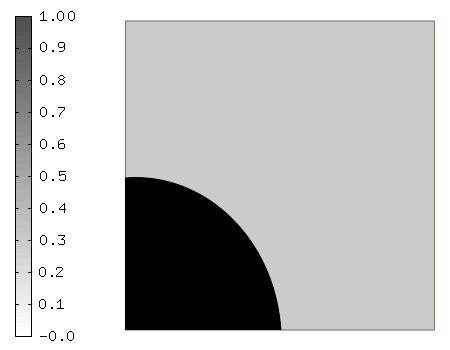
\includegraphics[width=0.48\textwidth]{Exact.png}
\label{fig:Exact}
\end{center}

\caption{Exact solution.}
\end{figure}
	
\subsection{Finite Volume Method}
We carry out the standard piecewise-constant finite volume discretization of the model problem using the \emph{upwinding} 
numerical flux \cite{compress}. The result corresponding to 32768 DOF is presented in Fig. 2.
\begin{figure}[H]
\begin{center}
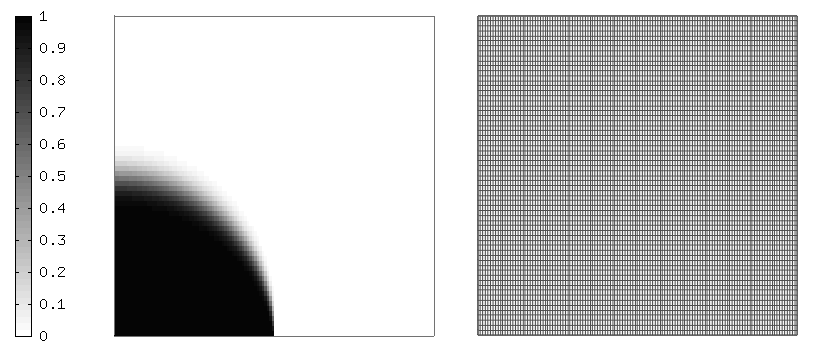
\includegraphics[width=0.9\textwidth]{fvm.png}
\label{fig:fvm000}
\end{center}

\caption{Approximation $u$ (left) and the corresponding mesh (right) with 32768 DOF. Relative L2 error 6.19\%.}
\end{figure}
\noindent
We can see that the solution is smeared near the steep gradient although a very fine mesh was used. 
	
\subsection{Finite Element Method}
In order to keep mesh granularity as well as the number of DOF similar to the previous FVM computation, we use linear elements. For
this demonstration, no stabilization or shock capturing were used. The approximation exhibits the well-known Gibbs 
phenomenon \cite{compress} manifested by spurious oscillations 
in the numerical solution that are visible in Fig. \ref{fig:fem000}.

\begin{figure}[H]
\begin{center}
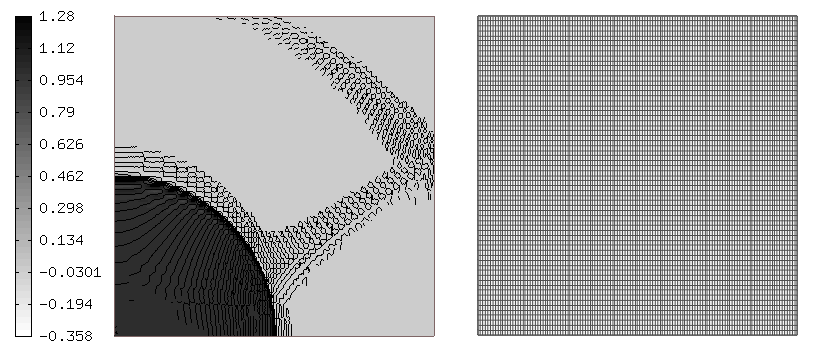
\includegraphics[width=0.9\textwidth]{fem.png}
\caption{Approximation $u$ (left) and the corresponding mesh (right) with polynomial degree $p = 1$ and 33153 DOF. 
Relative L2 error 7.24\%.}
\label{fig:fem000}
\end{center}
\end{figure}
\noindent
The oscillations can be reduced by employing a suitable stabilization technique such as the Streamline-Upwind Petrov-Galerkin (SUPG) method \cite{SUPG} or others. 

\subsection{Discontinuous Galerkin Method}
\label{sec:DG}
Since the DG discretization is still less frequently used compared to FVM and FEM, let us 
present briefly its derivation for our model problem. 
Let $\mc{T}_h$ be a triangulation of $\Omega$. For each $K\in\mc{T}_h$ we introduce the notation
\begin{eqnarray}
\partial K^- & = & \left\{x\in\partial K;\beta\lo\bs{x}\ro\cdot\bs{n}\lo\bs{x}\ro <0\right\},\\
\partial K^+ & = & \left\{x\in\partial K;\beta\lo\bs{x}\ro\cdot\bs{n}\lo\bs{x}\ro \geq 0\right\}.
\end{eqnarray}
By $H^k\lo\Omega, \mc{T}_h\ro$ we denote the so-called \itshape broken Sobolev space\upshape:
\be
H^k\lo\Omega,\mc{T}_h\ro = \left\{v\in L^2\lo\Omega\ro;\ v|_K\in H^k\lo K\ro \forall K\in \mc{T}_h\right\}.
\ee
For $u\in H^1\lo\Omega,\mc{T}_h\ro$ we set
\be
u_K^+ = \text{trace of } u|_K \text{ on }\partial K
\ee
(i.e., the interior trace of $u$ on $\partial K$). For each edge $E\subset\partial K\backslash\Gamma$ of $K$, there exists $K'\neq K,\ K'\in\mc{T}_h$, adjacent to $E$ and opposite to $K$. Then we put
\be
u_K^- = \text{trace of } u|_{K'} \text{ on } E.
\ee
In this way we obtain the exterior trace $u_K^-$ of $u$ on $\partial K\backslash\Gamma$ and define the jump of $u$ on $\partial K\backslash\Gamma$:
\be
[u]_K = u_K^+ - u_K^-.
\ee
Let $u\in H^1\lo\Omega\ro$ be a solution of the problem~\eqref{ade}. Then $u$ satisfies the identity
\be
\int_K \nabla\cdot\lo\beta u\ro\varphi d\bs{x} = 0,\ \ \varphi\in H^1\lo\Omega,\mc{T}_h\ro,\ K\in\mc{T}_h.
\ee
The application of Green's theorem gives
\begin{eqnarray}
\label{upwinding_derivation_ade}
\int_K \nabla\cdot\lo\beta u\ro\varphi d\bs{x} 
& = & \int_{\partial K}\lo\beta u_K^+\ro\cdot\bs{n}\varphi_K^+ dS - \int_K \lo\beta u\ro\cdot\nabla \varphi d\bs{x}\\\nonumber
& = & \int_{\partial K^-}\lo\beta u_K^+\ro\cdot\bs{n}\varphi_K^+ dS + \int_{\partial K^+}\lo\beta u_K^+\ro\cdot\bs{n}\varphi_K^+ dS\\\nonumber
& - & \int_K \lo\beta u\ro\cdot\nabla \varphi d\bs{x},
\end{eqnarray}
where $\bs{n}$ is the unit outer normal to the element boundary $\partial K$. As $u\in H^1\lo\Omega\ro$, we have $u_K^-|_{\partial K} = u_K^+|_{\partial K}$. Moreover, $u_K^-|_{\partial K^-\cap\Gamma_-}:=u|_{\partial K^-\cap\Gamma_-} = g$. 
Then we can write
\begin{eqnarray}
\int_K \nabla\cdot\lo\beta u\ro\varphi d\bs{x} & = & \int_{\partial K^-}\lo\beta u_K^-\ro\cdot\bs{n}\varphi_K^+ dS + \int_{\partial K^+}\lo\beta u_K^+\ro\cdot\bs{n}\varphi_K^+ dS\\\nonumber & - & \int_K \lo\beta u\ro\cdot\nabla \varphi d\bs{x}.
\end{eqnarray}
Applying Green's theorem again, we get the identity
\be
\label{DG_identity_ade}
\int_K \nabla\cdot\lo\beta u\ro\varphi d\bs{x} = \int_{\partial K^-}\lo\beta \lo u_K^+ - u_K^-\ro\ro\cdot\bs{n}\varphi_K^+ dS.
\ee
Setting
\begin{eqnarray}
a_K\lo u, \varphi\ro & = & \int_K \nabla\cdot\lo\beta u\ro\varphi d\bs{x} - \int_{\partial K^-\backslash\Gamma}\lo\beta [u]_K\ro\cdot\bs{n}\varphi_K^+ dS\\\nonumber & - & \int_{\partial K^-\cap\Gamma_-}\lo\beta u_K^+\ro\cdot\bs{n}\varphi_K^+ dS,
\end{eqnarray}
\be
L_K\lo\varphi\ro = \int_{\partial K^-\cap\Gamma_-}\lo\beta g\ro\cdot\bs{n}\varphi_K^+ dS,
\ee
we can rewrite the equation~\eqref{DG_identity_ade} as
\be
\label{final_DG_ade}
a_K\lo u, \varphi\ro = L_K\lo\varphi\ro,\ \ \varphi\in H^1\lo K\ro,\ \ K\in\mc{T}_h.
\ee
This identity makes sense also for $u\in H^1\lo\Omega, \mc{T}_h\ro$. In this case, we can note that in~\eqref{upwinding_derivation_ade}, on $\partial K^-$ (= the inlet of $K$ with respect to the velocity $\beta$) we replace the value $u_K^+$ (the interior trace of u) by $u_K^-$. This means that $upwinding$ is used here, because the value of the trace of $u$ on $\partial K^-$ is taken from the side of $\partial K^-$ against the velocity direction.

The approximate solution is a function $u_h$ satisfying the conditions
\begin{enumerate}
\item $u_h\in V_h = V^{p, -1}\lo\Omega,\mc{T}_h\ro:=\left\{\varphi\in L^2\lo\Omega\ro;\varphi|_K\in P^p\lo K\ro\forall K \in \mc{T}_h\right\}$
\item $a_K\lo u_h, \varphi_h\ro = L_K\lo\varphi_h\ro,\ \forall\varphi_h\in V_h,\ \forall K\in\mc{T}_h$.
\end{enumerate}
Here $p$ stands for the polynomial degree. In general, on each element a different polynomial degree can be used. The approximate solution and test functions are piecewise polynomial functions without any continuity requirement on interfaces between neighboring elements. The continuity requirement is replaced here by the jump term 
$$
\int_{\partial K^-\backslash\Gamma}\lo\beta [u]_K\ro\cdot\bs{n}\varphi_K^+ dS.
$$ 
The $hp$-DG discretization of the Euler equations will be presented in Section~\ref{sec:DGEuler}.
In Fig.~\ref{fig:DG_2} we can see that we successfully avoided the smeared layer close to the steep 
gradient as well as the Gibbs phenomenon in the whole domain. On the other hand, we have to deal with overshoots and undershoots close to the steep gradient that also render the relative L2 error higher. Here the issue was not addressed, for the comparison with the other two methods to be fair. 
There are several approaches how to solve this problem, some of which are described in the last chapter with 
numerical experiments, for the case of the Euler equations.

\begin{figure}[H]
\begin{center}
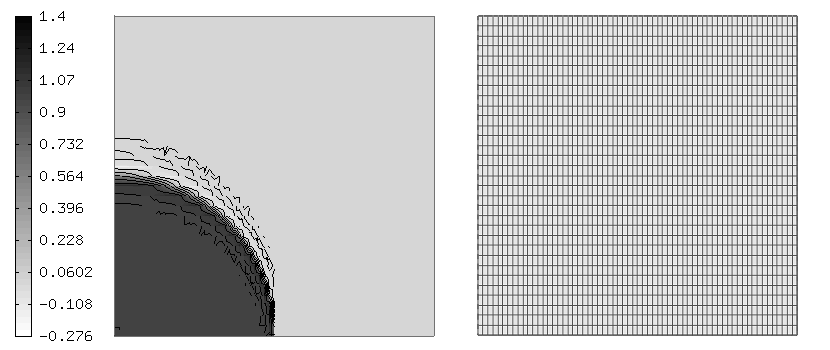
\includegraphics[width=0.9\textwidth]{dg.png}
\caption{Approximation $u$ (left) and the corresponding mesh (right) with polynomial degree $p = 1$ and 32768 DOF. Relative L2 error 8.89\%.}
\label{fig:DG_2}
\end{center}
\end{figure}

\section{Adaptive $hp$-DG with dynamically-changing meshes}

In this section we present the novel adaptivity algorithm that is the main contribution of the paper. The algorithm will be applied to Compressible Euler equations in Section 3. We refer to \cite{dubcova,multimesh1,multimesh2} for basic ideas of element-wise assembling in the $hp$-adaptivity settings. In particular, references \cite{dubcova,multimesh2} describe how \emph{multimesh assembling} is used to construct adaptive $hp$-FEM/$hp$-DG with dynamically changing meshes for transient PDE problems. In these articles, as well as in this work, we prefer to use Rothe's method to the method of lines for space-time discretization. The algorithms presented below are implementation-dependent and their concrete 
implementation can be found in the open source library Hermes \cite{hermes}.
\paragraph{Notation}
In the algorithm description, we shall use the following notation. Note that the description presented is for a scalar problem, vector problem differs only in the number of components.\\
\\
\begin{tabular}[t]{ll}
$time$&current (physical) time \\
$n$&current time step \\
$timeStep$&current length of (physical) time step\\
$\mathbf{Space}_n$&DGFE space at time step $n$\\
$\mathbf{SpaceCoarse}_n$&\emph{coarse space}(see below) at time step $n$\\
$\mathbf{Mesh}_n$&mesh (corresponding to $\mathbf{Space}_n$) at time step $n$\\
$\mathbf{Solution}_n$&solution at time step $n$\\
$\mathbf{SolutionCoarse}_n$&$\mathbf{Solution}_n$ projected on $\mathbf{SpaceCoarse}_n$\\
$\mathbf{error}$&calculated relative error estimate\\
$\mathbf{errorTol}$&error estimate tolerance (see below)
\end{tabular}
\paragraph{Algorithm}
This is the algorithm of the solution of Non-stationary Compressible Euler equations using $hp$-DG. Some terms are marked with a number in square brackets. These terms are explained more thoroughly after the algorithm outline under the appropriate number.
\begin{enumerate}
\item
Initialization:
\begin{itemize}
\item $timeStep$ = a very small initial time step
\item $\mathbf{Space}_1 = \mathbf{Space}_0$ = initial DGFE space - may be very coarse
\item $\mathbf{Solution}_0$ = set according to the initial condition
\item $n$ = 1
\item $time$ = 0.0
\end{itemize}
\item Time-stepping loop:
\begin{enumerate}
\item  Conditionally invoked global mesh de-refinement$^{\mathbf{[1]}}$.
\item  Adaptivity loop:
\begin{enumerate}
\item  Assemble$^{\mathbf{[2]}}$ and solve the linear problem on $\mathbf{Space}_n$ obtaining $\mathbf{Solution}_n^{\mathbf{[3]}}$.
\item  (DG specific): detect discontinuities and limit solution $\mathbf{Solution}_n$ to prevent the Gibb's phenomenon.
\item  Project the (limited) $\mathbf{Solution}_n$ to \emph{coarse space} $\mathbf{SpaceCoarse}_n$ $^{\mathbf{[4]}}$ to obtain $\mathbf{SolutionCoarse}_n$.
\item  Calculate error estimate$^{\mathbf{[5]}}$, per element (for adaptivity) and global - $\mathbf{error}$.
\item  is $\mathbf{error}\ <\ \mathbf{errorTol}$ ?
\begin{itemize}
\item (YES)  \begin{enumerate}
\item  As the $\mathbf{Solution}_n$ is captured with the desired tolerance, go to (c).
\end{enumerate}
\item (NO) \begin{enumerate}
\item  Adapt the $\mathbf{Space}_n$.
\begin{itemize}
\item Select elements for refinement$^{\mathbf{[6]}}$
\item For each of the elements selected for refinement, select the optimal $hp$-refinement candidate$^{\mathbf{[7]}}$.
\end{itemize}
\item  Go to (a) - calculate on the adapted space $\mathbf{Space}_n$.
\end{enumerate}
\end{itemize}
\end{enumerate}
\item  Calculate new $timeStep$ value based e.g. on CFL condition.
\item  Set $time = time + timeStep\ \ \ n = n + 1$.
\end{enumerate}
\end{enumerate}

\begin{center}
\line(1,0){450}
\end{center}
$\mathbf{[1]}$ \textbf{Global mesh de-refinement} Conditions include e.g. number of DOFs, number of adaptive steps or time steps since last de-refinement etc.\\\ \\
The Hermes library offers three options of global de-refinement:\\
\begin{itemize}
\item Reset the mesh $\mathbf{Mesh}_n$ to a coarse base mesh $\mathbf{Mesh}_{base}$. Reset the 
      polynomial degrees of all elements to the initial polynomial degree $p_{init}$.
\item Remove $m$ refinement layers uniformly from all elements in the mesh $\mathbf{Mesh}_n$. Here $m$ 
      is usually one, two or at most three. Here the refinements can be anisotropic, and the internal structures facilitate the removing of such layers in the same fashion as isotropic refinements. Reset the polynomial degrees of all elements
      to the initial polynomial degree $p_{init}$.
\item Remove just one refinement layer uniformly from all elements in the mesh $\mathbf{Mesh}_n$. 
      Decrease the polynomial degrees of all mesh elements by one.
\end{itemize}
The first option is mathematically the cleanest, meaning that the mesh obtained 
on the new time level are completely independent from the mesh that was
generated during the last time step. The last option is the fastest, but the 
sequence of dynamical meshes generated in this way may have on average 
more DOFs than is needed. The second option is a compromise.\\\ \\
$\mathbf{[2]}$ \textbf{Assembling of the problem} The $hp$-DG assembling requires treating several difficulties:
\begin{itemize}
\item hanging nodes: increases the difficulty of searching for element's neighbors for calculating numerical fluxes
\item variable polynomial degree: damaged sparsity pattern of the matrix
\item projection-based error estimation: treating overshoots and undershoots very well is a must, otherwise $\mathbf{Solution}_n$ can not be treated as the 'reference' solution.
\end{itemize}
$\mathbf{[3]}$ \textbf{Dynamical meshes} It is noteworthy that one has to use $\mathbf{Solution}_{n-1}$ for the calculation of $\mathbf{Solution}_n$ here.
These solutions, however, are generally defined in different spaces: $\mathbf{Space}_{n}, \mathbf{Space}_{n-1}$, and therefore, projections, or the \emph{multimesh} assembling (see above), must be used.\\\ \\
$\mathbf{[4]}$ \textbf{Projection to \emph{coarse space} $\mathbf{SpaceCoarse}_n$} Here, the \emph{coarse space} is a DGFE space used for error estimate calculation with the following origin: the (reference) space is created from this \emph{coarse space} by uniform mesh refinement and global increase of polynomial degree by 1.\\\ \\
$\mathbf{[5]}$ \textbf{Error estimation} Both global and element-wise relative error estimate is calculated using the following:
	$$error_{estimate} = \frac{\mathbf{Solution}_{n} - \mathbf{SolutionCoarse}_n}{\mathbf{Solution}_{n}}$$
$\mathbf{[6]}$  \textbf{$hp$-refinement strategy} As the goal of the adaptivity is to find an "optimal" $\mathbf{Space}_n$ for capturing ${\mathbf{Solution}_{n}}$, we have to apply a strategy to determine what elements to refine based on the calculated element-wise errors. One of the usual strategies is e.g. to refine only top fraction of elements sorted by their error in descending order. More about these strategies can be found in the literature cited before.\\\ \\
$\mathbf{[7]}$  \textbf{Selecting optimal $hp$-refinement}
Some implementation of the algorithm for determining optimal $hp$-refinements, such as in \cite{derade}, are 
quite complex. Built upon the projection-based interpolation theory,
such approach first finds optimal $hp$-refinement of mesh edges using a 1D
version of the $hp$-adaptive algorithm. The edge refinements then
determine $h$-refinement of elements. Finally, best polynomial
degrees for element interiors are selected. Each step of the algorithm
represents a considerable implementation burden.

We have implemented a much simpler scheme, which is local in the sense
that element refinements are selected without regard to the refinements
of neighboring elements. For all elements $K\in \mathbf{Mesh}_n$ of polynomial
degree $p$ picked by the outer loop we consider the following 
$N = 83$ $hp$-refinement options:
\begin{enumerate}
\item Increase the polynomial degree of $K$ to $p+1$ without spatial subdivision.
\item Increase the polynomial degree of $K$ to $p+2$ without spatial subdivision.
\item Split $K$ into four similar triangles $K_1, K_2, K_3, K_4$.
      Define $p_0$ to be the integer part of $(p+1)/2$.
      For each $K_i$, $1 \le i \le 4$ consider polynomial
      degrees $p_0 \le p_i \le p_0 + 2$.
\end{enumerate}
For each of these $N$ options we perform a standard element-bound $L_2$-projection
of the reference solution $\mathbf{Solution}_{n}$ onto the space of polynomials defined on the element, corresponding to the candidate. The most suitable candidate (selection based on the projection error and added DOFs) is selected for $hp$-refinement of the element $K$.\\

Each of the $N$ projection problems requires the solution of a small
system of linear algebraic equations with a symmetric positive-definite
matrix. The solution of these systems can be further optimized by exploiting
the incremental nature of the Cholesky decomposition algorithm 
and the fact that the spaces in item 3 above are partially embedded. 

\begin{center}
\line(1,0){450}
\end{center}

\paragraph{Example}
We again solve Problem~\ref{ade} but this time, we shall start with a very coarse initial mesh and automatic $hp$-adaptivity will be used. Although the maximum value of the exact solution is $1.0$, due to the presence of undershoots and overshoots, the maximum values here are higher, as was seen already in Section~\ref{sec:DG}. This can be avoided by using a suitable shock capturing method, as it is done in the last chapter with numerical examples for the Euler equations.
\vspace{-4mm}
\begin{figure}[H]
\begin{center}
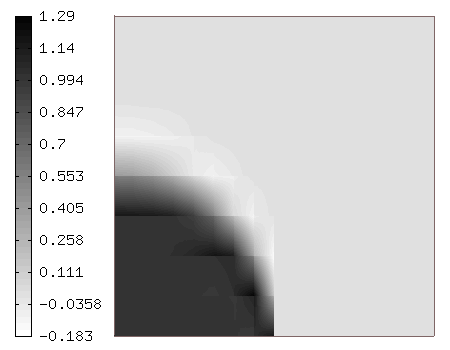
\includegraphics[width=0.45\textwidth]{ASln1.png}\ \ \ 
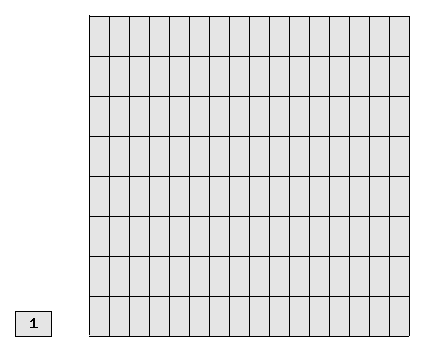
\includegraphics[width=0.44\textwidth]{Space1.png}
\end{center}
\vspace{-2mm}
\caption{Solution $\mathbf{Solution}_1$ calculated on the initial space $\mathbf{Space}_1$ polynomial degrees having 512 DOFs, $error_{estimate} = 25.77\%$.}
\end{figure}
\vspace{-10mm}
\begin{figure}[H]
\begin{center}
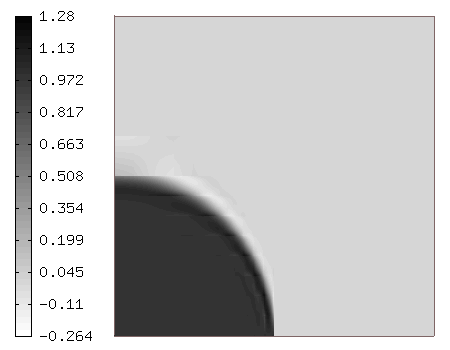
\includegraphics[width=0.45\textwidth]{ASln2.png}\ \ \ 
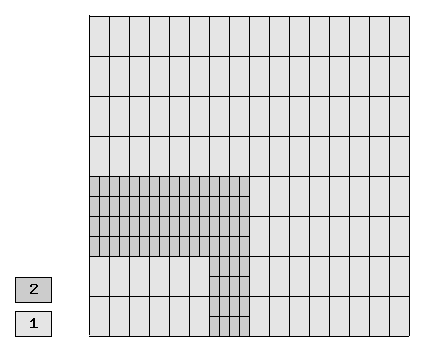
\includegraphics[width=0.44\textwidth]{Space2.png}
\end{center}
\vspace{-2mm}
\caption{Solution $\mathbf{Solution}_3$ and the space $\mathbf{Space}_3$ with polynomial degrees having 1152 DOFs, $error_{estimate} = 9.60\%$.}
\end{figure}
\vspace{-10mm}
\begin{figure}[H]
\begin{center}
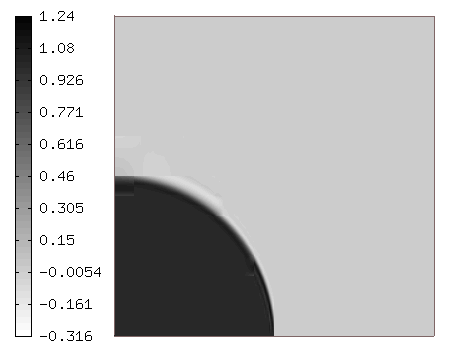
\includegraphics[width=0.45\textwidth]{ASln3.png}\ \ \ 
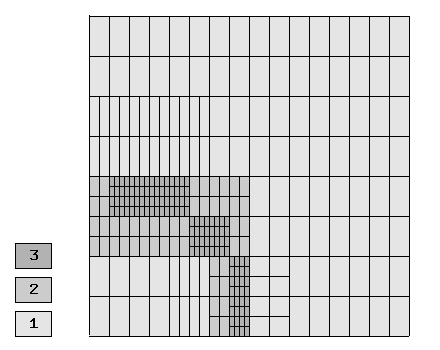
\includegraphics[width=0.44\textwidth]{Space3.png}
\end{center}
\vspace{-2mm}
\caption{Solution $\mathbf{Solution}_5$ and the space $\mathbf{Space}_5$ with polynomial degrees having 2992 DOFs, $error_{estimate} = 4.46\%$.}
\end{figure}
\vspace{-2mm}
\begin{figure}[H]
\begin{center}
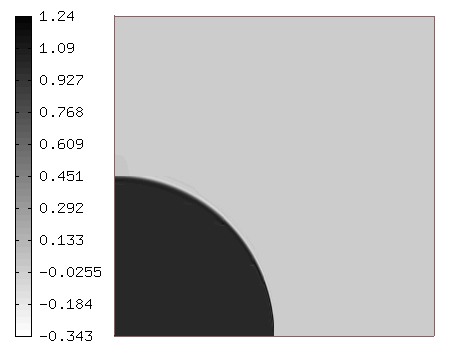
\includegraphics[width=0.45\textwidth]{ASln4.png}\ \ \ 
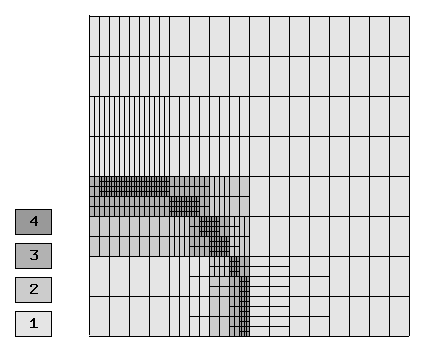
\includegraphics[width=0.44\textwidth]{Space4.png}
\end{center}
\vspace{-2mm}
\caption{Final solution $\mathbf{Solution}_7$ and the space $\mathbf{Space}_7$ with polynomial degrees having 9872 DOFs, $error_{estimate} = 2.32\%$.}
\end{figure}

\section{Discontinuous Galerkin discretization of the Euler equations}
\label{sec:DGEuler}
This section describes only important parts of the process of DG discretization of the Euler equations. The description of the semi-implicit time integration (\cite{DF04}), and linearization, are omitted here.
\subsection{Discontinuous Galerkin space semidiscretization}
We approximate the Euler fluxes $\f_1, \f_2$ (\cite{compress}) through the element faces $\Gamma_{ij}$, between elements $K_i$ and $K_j$, where $K_i, K_j\in\mc{T}_h$, with the aid of a numerical flux $\bs{H}=\bs{H}(\uu,\w,\nn)$ in the form
\begin{equation} \label{eq:5}
\int_{\Gamma_{ij}}  \sum_{s=1}^2\,\f_s(\w(t))\,{(n_{ij})}_s\cdot \boldsymbol{\varphi}_h \,d S
 \approx
\int_{\Gamma_{ij}} 
\bs{H}(\w_h(t)|_{K_i}, \w_h(t)|_{K_j},\nn_{ij})\cdot\boldsymbol{\varphi}_h\,d S,
\end{equation}
where $\nn_{ij}$ is the unit outer normal to $K_i$.

\subsection{Numerical fluxes}
  The DGFEM discretization of the Euler equations in their conservative form follows the principles of the section~\ref{sec:DG}.
We define
\be
\mathbb{A}_s\lo\bs{w}\ro = \frac{D\bs{f}_s\lo\bs{w}\ro}{D\bs{w}},\ 
\mc{P}\lo\bs{w},\bs{n}\ro = \sum_{s = 1}^{2}\bs{f}_s\lo\bs{w}\ro n_s,
\ee
where the latter is the flux of the quantity $\bs{w}$ in the direction $\bs{n}$. The Jacobi matrix $D\mc{P}\lo\bs{w},\bs{n}\ro/D\bs{w}$ can be expressed in the form
\be
\frac{D\mc{P}\lo\bs{w},\bs{n}\ro}{D\bs{w}} = \mathbb{P}\lo\bs{w},\bs{n}\ro = \sum_{s=1}^2\mathbb{A}_s\lo\bs{w}\ro n_s.
\ee
See~\cite{1993} for details. The following numerical fluxes were used in calculations.
\ \\
\begin{enumerate}
\item \emph{The Steger-Warming scheme} has the numerical flux:
$$ \bs{H}_{SW}\lo\bs{u},\bs{v},\bs{n}\ro = \mathbb{P}^+\lo\bs{u},\bs{n}\ro\bs{u} + \mathbb{P}^-\lo\bs{v},\bs{n}\ro\bs{v},\ \ \bs{u},\bs{v}\in D,\ \bs{n}\in\mc{S}_1.$$
This scheme turned out to be rather diffusive, therefore another scheme is preferred.\newline
\item  \emph{The Vijayasundaram scheme} has the numerical flux:
$$ \bs{H}_{V}\lo\bs{u},\bs{v},\bs{n}\ro = \mathbb{P}^+\lo\frac{\bs{u} + \bs{v}}{2},\bs{n}\ro\bs{u} + \mathbb{P}^-\lo\frac{\bs{u} + \bs{v}}{2},\bs{n}\ro\bs{v},\ \ \bs{u},\bs{v}\in D,\ \bs{n}\in\mc{S}_1.$$
\end{enumerate}

\subsection{Boundary conditions}
\label{sec:bnd}
In both examples in the next chapter, the boundary of the computational domain $\Omega$ is divided into three parts.
\begin{enumerate}
\item On a fixed impermeable wall $\Gamma_W\subset\partial\Omega$ we use the condition $\bs{v}\cdot\bs{n} = 0$. Then the flux $\mc{P}\lo\bs{w},\bs{n}\ro$, defined as $\sum_{s=1}^2\mathbb{A}_s\lo\bs{w}\ro n_s$, has the form
\begin{eqnarray}
\mc{P}\lo\bs{w},\bs{n}\ro & = & \sum_{s=1}^2\bs{f}_s\lo\bs{w}\ro n_s \\ & = & \lo\bs{v}\cdot\bs{n}\ro\bs{w} + p \lo 0, n_1, n_2, \bs{v}\cdot\bs{n}\ro^T \\ & = & p\lo 0, n_1, n_2, 0\ro^T,
\end{eqnarray}
which is uniquely determined on $\Gamma_W$ by the extrapolated value of the pressure, i.e. by $p_j^k := p_i^k$. Therefore, on the part $\Gamma_W$ of the boundary we define the numerical flux
\be
\bs{H}\lo\bs{w}_i^k, \bs{w}_j^k, \bs{n}\ro = p_i^k\lo 0, n_1, n_2, 0\ro^T.
\ee
On the impermeable part of the boundary, we prescribe only $\bs{v}\cdot\bs{n} = 0$, and extrapolate the pressure. For details, see~\cite{hyp06}.
\item
On the inlet
$$
\Gamma_I\lo t \ro = \left\{x\in\partial\Omega; \bs{v}\lo x, t\ro \cdot \bs{n}\lo x \ro < 0\right\}
$$
and the outlet
$$
\Gamma_O\lo t \ro = \left\{x\in\partial\Omega; \bs{v}\lo x, t\ro \cdot \bs{n}\lo x \ro > 0\right\}
$$
parts of the boundary it is necessary to use nonreflecting boundary conditions. In this case we used the so-called \emph{characteristics-based} boundary conditions, according to~\cite{hyp06}.
\end{enumerate}
\subsection{Shock capturing}
\label{subsec:shock}
For the flow containing discontinuities we need to employ suitable stabilization technique to avoid spurious overshoots and undershoots in computed solutions near the discontinuities. This phenomenon does not occur in low Mach number regimes, but in transonic flow it causes instabilities in the numerical solution.
\paragraph{}
Two approaches will be presented and later used in the numerical examples. The first one, the so-called \emph{vertex based limiter} is taken from~\cite{Kuzmin}. The second one, based on adding \emph{artificial viscosity} into the system of equations is taken from~\cite{hyp06}. Both were used for a variety of numerical examples and turned out to work well. For obtaining the results presented in the last section, the \emph{vertex based limiter} was used.
\subsubsection{Vertex based limiter}
\label{sec:vertex_limiter}
The vertex based limiter is based on a simple idea of limiting the slope of the solution on an element by limiting
the polynomial degree of approximation used on that element. Let $v$ be a component of the numerical solution. Given an element $K_i\in\mc{T}_h$, the value of the solution on $K_i$ in the center of gravity of $K_i$, denoted by $v^c_i$, and the average value of the gradient of the solution in the center of gravity, denoted by $\lo\nabla v\ro^c_i$, the goal is to determine the maximum admissible slope for a constrained reconstruction of the form
\be
\label{corr_factors}
v_h\lo\bs{x}\ro = v^c_i +\alpha_i\lo\nabla v\ro^c_i \cdot \lo\bs{x} - \bs{x}^c_i\ro,\ \ 0\leq\alpha_i\leq 1,\ \bs{x}\in K_i,
\ee
where $\bs{x}^c_i$ is the center of gravity of $K_i$. The correction factor $\alpha_i$ is defined so that the final solution values at the vertices of $K_i$, denoted in what follows as $\bs{x}_{i,j},\ j = 1, ...,\mbox{ number of vertices}$, are bounded by the maximum and minimum values of $v$ in all elements sharing the vertex $\bs{x}_{i,j}$. We define these values as $v_{i,j}^{\max}, v_{i,j}^{\min}$.

The element-wise correction factors $\alpha_i$ for~\ref{corr_factors} guarantee that
\be
v_{i,j}^{\min}\leq v\lo\bs{x}_{i,j}\ro\leq v_{i,j}^{\max},\ \forall j.
\ee
This vertex-based condition can be enforced using
\be
\alpha_i = \min_j
\begin{cases}
\min\left\{1,\frac{v_{i,j}^{\max} - v^c_i}{v\lo\bs{x}_{i,j}\ro - v^c_i}\right\},\ \mbox{if } v\lo\bs{x}_{i,j}\ro - v^c_i > 0,\\
1,\\
\min\left\{1,\frac{v_{i,j}^{\min} - v^c_i}{v\lo\bs{x}_{i,j}\ro - v^c_i}\right\},\ \mbox{if } v\lo\bs{x}_{i,j}\ro - v^c_i < 0.\\
\end{cases}
\ee
Higher order terms are handled using similar ideas.

\subsubsection{Limiter based on adding artificial viscosity}
\label{sec:limiter_feist}
First part of this approach is introducing the discontinuity indicator $g\lo i \ro$ proposed in~\cite{DFS03} and defined by
\be
g\lo i \ro = \int_{\partial K_i}\left[\rho_h^k\right]^2 dS / \lo h_{K_i}|K_i|^{3/4}\ro,\ K_i\in\mc{T}_h.
\ee
Further we define the discrete indicator
\be
G\lo i \ro = 0 \mbox{ if } g\lo i \ro <1 \mbox{ and } G\lo i \ro = 1 \mbox{ if } g\lo i \ro \geq 1,\ \ K_i\in\mc{T}_h.
\ee
To the left hand-side of the linearized equations (see~\cite{DF04}), we add the \emph{artificial viscosity forms}
\be
\beta_h\lo\bs{w}_h^k, \bs{w}_h^{k+1},\boldsymbol{\varphi}\ro = \nu_1\sum_{i\in I} h_{K_i} G^k\lo i \ro \int_{K_i}\nabla\bs{w}_h^{k+1}\cdot\nabla\boldsymbol{\varphi} d\bs{x}
\ee
and
\be
J_h\lo\bs{w}_h^{k},\bs{w}_h^{k+1},\boldsymbol{\varphi}\ro = \nu_2\sum_{i\in I}\sum_{j\in s\lo i \ro}\frac12\lo G^k\lo i \ro + G^k\lo j\ro\ro\int_{\Gamma_{ij}}\left[\bs{w}_h^{k+1}\right]\cdot\left[\boldsymbol{\varphi}\right] dS,
\ee
where $\nu_1, \nu_2 \approx 1$.
An important characteristic of this approach is that $G\lo i \ro$ vanishes in regions, where the solution is regular. Therefore, the scheme does not produce any nonphysical entropy in these regions.


\section{Numerical experiments}
We carry out numerical experiments for the non-stationary compressible Euler equations. On these examples we want to demonstrate the combination of $hp$-DG and Dynamical meshes.
The purpose of the first of the two examples presented is to verify the method and its ability to capture shock waves in flows in high Mach number regimes. In all numerical experiments, we consider the CFL stability condition of the form
\be
\tau_k\max_{K_i\in\mc{T}_h}\frac{1}{|K_i|}\lo\max_{j\in S\lo i \ro} |\Gamma_{ij}|\lambda_{\mc{P}\lo\bs{w}_h^k|_{\Gamma_{ij}}, \bs{n}_{ij}\ro}^{\max}\ro\leq CFL.
\ee
Here, $CFL$ is a given constant and $\lambda_{\mc{P}\lo\bs{w}_h^k|_{\Gamma_{ij}}, \bs{n}_{ij}\ro}^{\max}$ is the maximum over $\Gamma_{ij}$ of the spectral radius of the matrix $\mc{P}\lo\bs{w}_h^k|_{\Gamma_{ij}}, \bs{n}_{ij}\ro$.
\paragraph{}
Also in all numerical experiments, we consider the medium in which we study the flow to be the air, and therefore we set $\kappa = 1.4$.
\paragraph{}
In the light of~\ref{sec:bnd}, the prescribed boundary states are derived from primitive variables denoted as $\rho_{Ext},
 {v_{1}}_{Ext}, {v_{2}}_{Ext}, p_{Ext}$ using the transformations to the conservative variables.

\subsection{Flow in a channel}
These examples demonstrate transonic flows with high Mach numbers, where the application of shock capturing is crucial.
\subsubsection{Reflected shock benchmark}
This is a classic benchmark for the solution of compressible flow described in~\cite{reflected}.
The prescribed relative tolerance $\mathbf{errorTol}$ for guiding the $hp$-adaptivity was set to $0.5\%$.
There are two different prescribed boundary states for two inflow regimes, corresponding to the left (denoted with $^{Left}$), and to the top (denoted with $^{Top}$) part of the boundary, and are derived from the following prescribed values
\begin{eqnarray}
{\rho_{}}_{Ext}^{Left} & = & 1.0 \\
{v_{1}}_{Ext}^{Left} & = & 2.9 \\
{v_{2}}_{Ext}^{Left} & = & 0.0 \\
p_{Ext}^{Left} & = & 0.714286 \\
\\
\rho_{Ext}^{Top} & = & 1.7 \\
{v_{1}}_{Ext}^{Top} & = & 2.619334 \\
{v_{2}}_{Ext}^{Top} & = & -0.5063 \\
p_{Ext}^{Top} & = & 1.52819.
\end{eqnarray}
The initial state is chosen to be the one prescribed on the left part of the boundary (denoted with $^{Left}$).
The bottom part of the boundary is a solid wall, and the right part is outflow, with respective corresponding boundary conditions.
In the solution of this problem, we employed the shock capturing scheme described in~\ref{sec:vertex_limiter}.

In Figs.~\ref{fig:rs-1} -~\ref{fig:rs-4}, the solution and corresponding meshes with polynomial degrees differentiated by the color, at various time levels are shown.

\begin{figure}[H]
\begin{center}
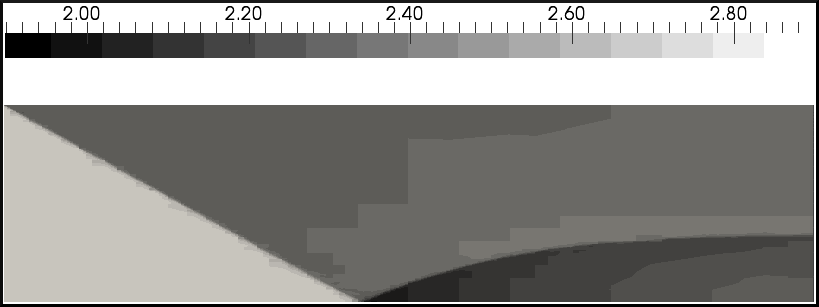
\includegraphics[width=\textwidth]{rs_sln.png}\ \ \ 
\end{center}

\caption{Solution: Mach number distribution, time = 1.0486s.}

\label{fig:rs-1}
\end{figure}

\begin{figure}[H]
\begin{center}
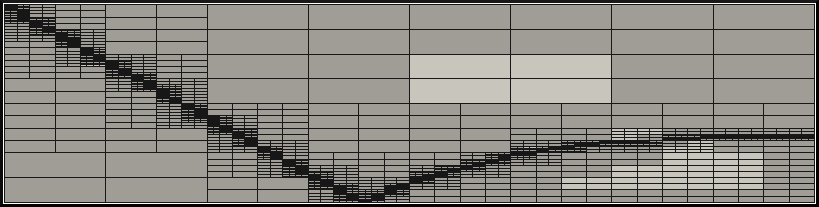
\includegraphics[width=\textwidth]{rs_mesh.png}\ \ \ 
\end{center}

\caption{Mesh, time = 1.0486s, number of DOFs: 17156.}

\label{fig:rs-2}
\end{figure}

\begin{figure}[H]
\begin{center}
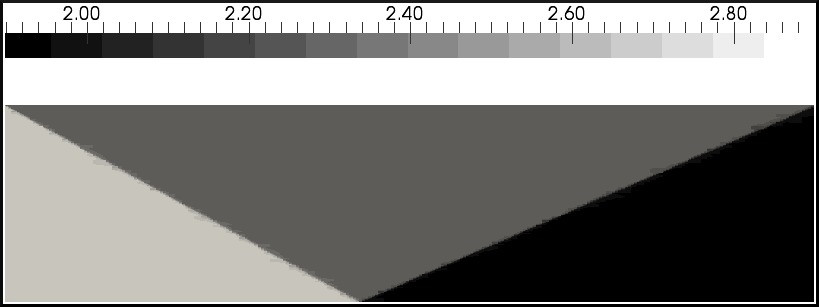
\includegraphics[width=\textwidth]{rs_finalSln.png}\ \ \ 
\end{center}

\caption{Final solution: Mach number distribution.}

\label{fig:rs-3}
\end{figure}

\begin{figure}[H]
\begin{center}
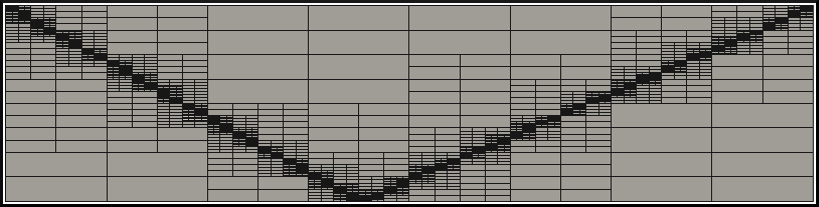
\includegraphics[width=\textwidth]{rs_finalMesh.png}\ \ \ 
\end{center}

\caption{Final mesh, number of DOFs: 30184.}

\label{fig:rs-4}
\end{figure}

In Fig.~\ref{fig:rs-11}, the same comparison to the exact solution, as in~\cite{reflected} was carried out, with good results.
\begin{figure}[H]
\begin{center}
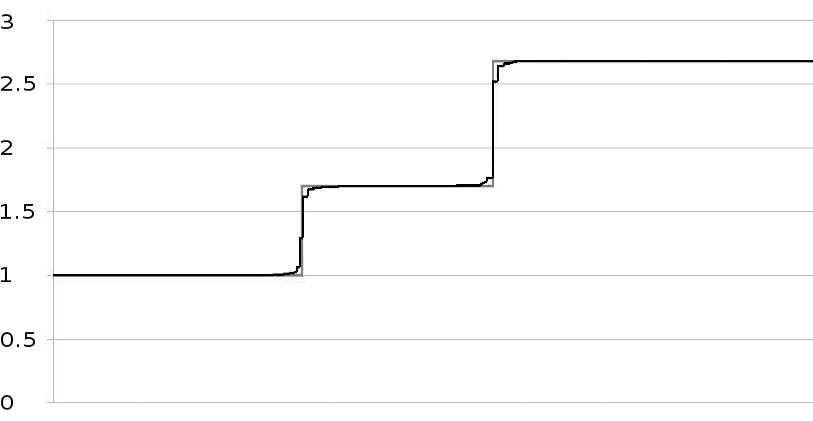
\includegraphics[width=0.7\textwidth]{density.png}\ \ \ 
\end{center}

\caption{Density along the line y = 0.25, exact solution (light), and calculated solution (dark). See~\cite{reflected}, Fig. 4, for comparison}

\label{fig:rs-11}
\end{figure}

\subsubsection{Forward facing step}
This is a classic benchmark for the solution of compressible flow.
In the light of~\ref{sec:bnd}, the prescribed boundary state is derived from the following prescribed values.
\begin{eqnarray}
\rho_{Ext} & = & 1.4 \\
{v_{1}}_{Ext} & = & 3.0 \\
{v_{2}}_{Ext} & = & 0.0 \\
p_{Ext} & = & 1.0
\end{eqnarray}
The left part of the boundary is an inlet part, whereas the right part is an outlet. The rest of the boundary is formed by solid walls.
The initial state is chosen to be the one prescribed on the left part of the boundary.
In the solution of this problem, we again employed the shock capturing scheme described in~\ref{sec:vertex_limiter}.
The prescribed relative tolerance $\mathbf{errorTol}$ for guiding the $hp$-adaptivity was set to $3.0\%$, later decreased to $2.0\%$ to capture the solution development.
In Figs.~\ref{fig:ffs-1} -~\ref{fig:ffs-4}, the solution and corresponding meshes with polynomial degrees differentiated by the color, at various time levels are shown.
\begin{figure}[H]
\begin{center}
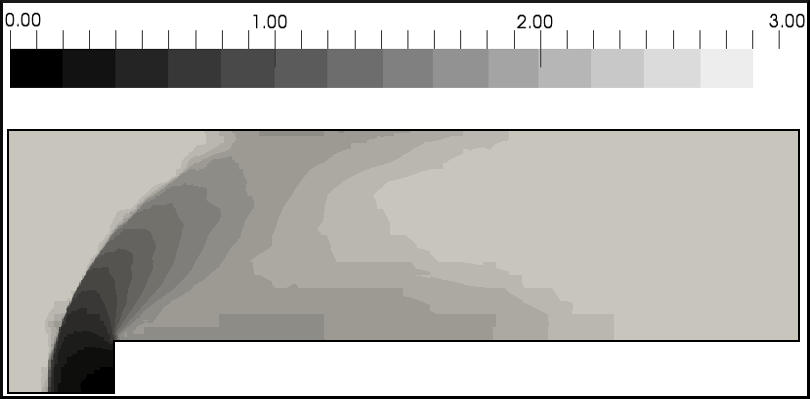
\includegraphics[width=0.7\textwidth]{sln1.png}\\
\vspace{2mm}
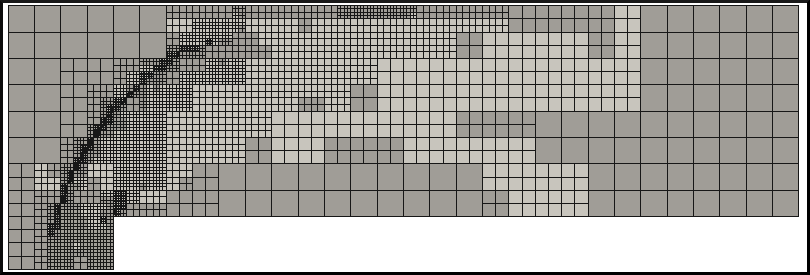
\includegraphics[width=0.7\textwidth]{mesh1.png}
\end{center}
\caption{Solution (Mach number distribution), and mesh, time = 0.616281.}
\label{fig:ffs-1}
\end{figure}

\begin{figure}[H]
\begin{center}
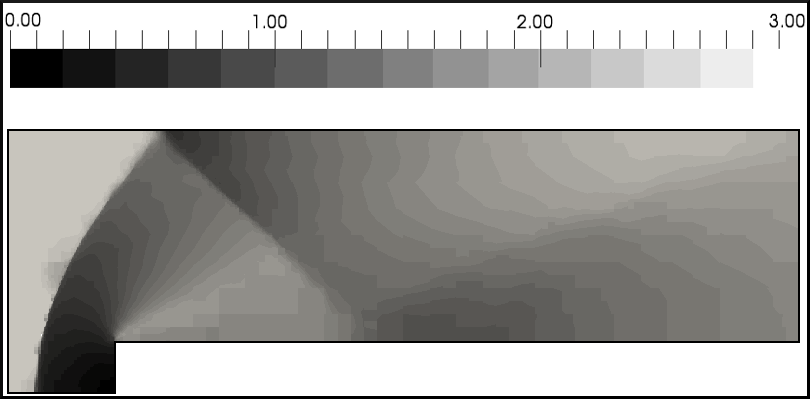
\includegraphics[width=0.7\textwidth]{sln2.png}\\
\vspace{2mm}
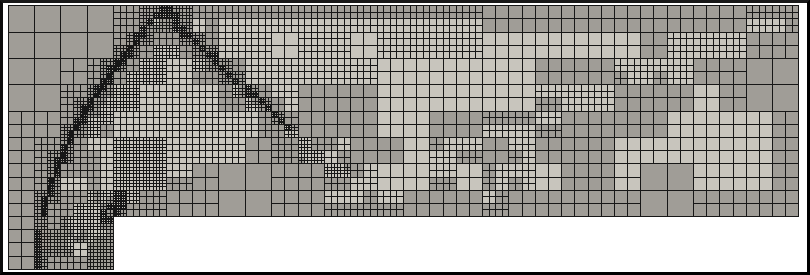
\includegraphics[width=0.7\textwidth]{mesh2.png}
\end{center}
\caption{Solution (Mach number distribution), and mesh, time = 2.07892.}
\label{fig:ffs-2}
\end{figure}

\begin{figure}[H]
\begin{center}
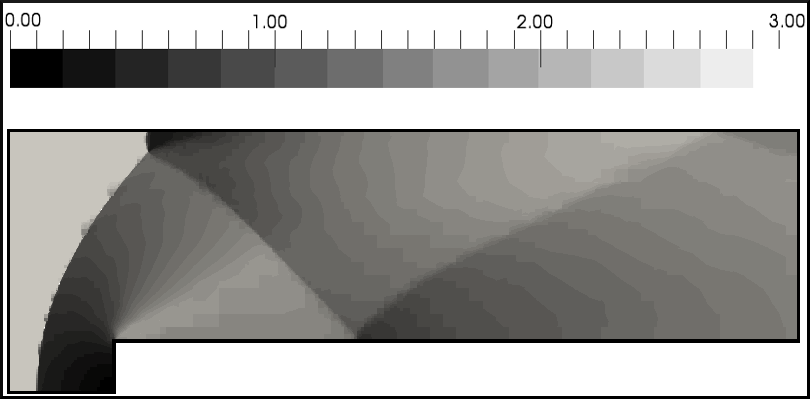
\includegraphics[width=0.7\textwidth]{sln3.png}\\
\vspace{2mm}
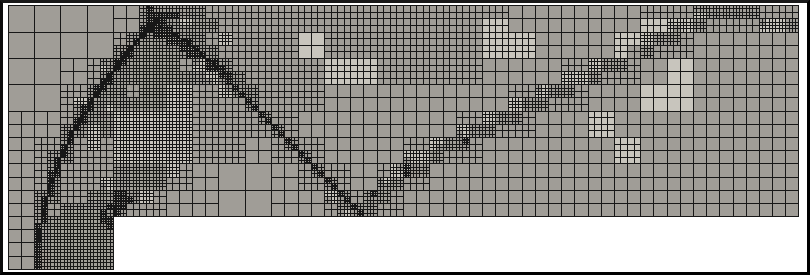
\includegraphics[width=0.7\textwidth]{mesh3.png}
\end{center}
\caption{Solution (Mach number distribution), and mesh, time = 2.87897.}
\label{fig:ffs-3}
\end{figure}

\begin{figure}[H]
\begin{center}
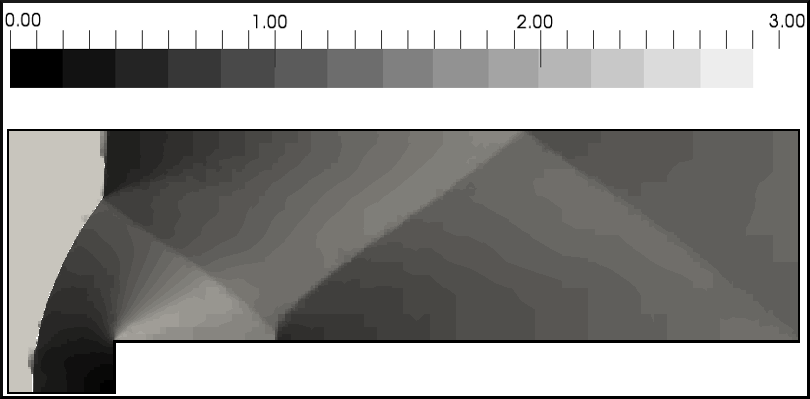
\includegraphics[width=0.7\textwidth]{sln4.png}\\
\vspace{2mm}
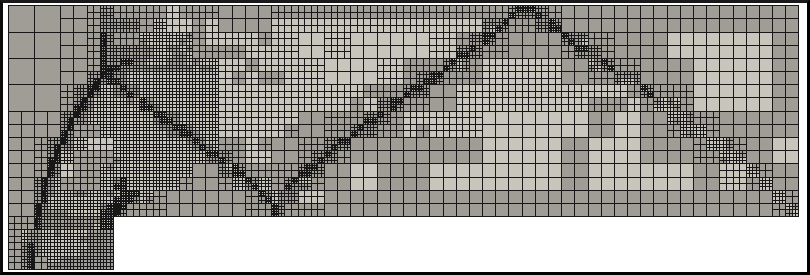
\includegraphics[width=0.7\textwidth]{mesh4.png}
\end{center}
\caption{Solution (Mach number distribution), and mesh, time = 3.5648.}
\label{fig:ffs-4}
\end{figure}

\section*{Conclusion and Outlook}

The main contribution of this paper is a novel adaptive algorithm for time-dependent compressible Euler 
equations solved by the $hp$-DG method. The algorithm uses meshes that change dynamically in time,
and thus it is suitable for problems where traveling shock waves are present.  
The algorithm was described and successfully applied to non-stationary compressible Euler equations.
The findings made during this research indicate that the following issues should be addressed in 
the future:

\begin{enumerate}
\item The semi-implicit scheme, that we expected to be unconditionally stable, does not behave in this 
way for all problems. Some time-dependent problems require the time step to be rather small in order 
to satisfy the CFL condition. Further analysis of stability of this method is desirable and fully implicit 
schemes should be studied.
\item One has to be aware of the fact that additional challenges for $hp$-adaptivity algorithms arise
in 3D -- there are more ways to refine an element, more integration points for higher order elements, more
complicated structure of constraints in arbitrary-level hanging nodes, etc.
\item Although $hp$-DG algorithms in the Hermes library utilize parallel computation in the shared memory 
environment, the use of domain decomposition and parallelization will be need to solve large 3D problems.
\end{enumerate}


\section*{Acknowledgment}

This research was supported by the following sources:
\begin{enumerate}
\item the European Regional Development Fund and the Ministry of
Education, Youth and Sports of the Czech Republic under the Regional Innovation Centre for Electrical
Engineering (RICE), project No. CZ.1.05/2.1.00/03.0094
\item Grant No. P105/10/1682 of the Grant Agency of the Czech Republic
\item Subcontract No. 00089911 of Battelle Energy Alliance (U.S. Department of Energy intermediary)
\item SGS (Studentska Grantova Soutez) grant number SGS-2012-039
\end{enumerate}


\begin{thebibliography}{99}
\addcontentsline{toc}{section}{Bibliography}

\bibitem{Babuska}Babuska I., Prager M., Vitasek E.: {\em Numerical Processes in Differential Equations}, STNL Praha - Wiley, 1966.

 \bibitem{demk1}
Demkowicz L., Oden J.T., Rachowicz W., Hardy O.:
Toward a universal $hp$-adaptive finite element strategy.
Part 1: constrained approximation and data structure.
Comput. Methods Appl. Math. Engrg., \textbf{77}, 79 - 112, 1989.

\bibitem{cerveny}
Cerveny, J., higher-order adaptive FEM for non-linear coupled problems, Department of Mathematical Sciences, The University of Texas at El Paso, 2007

\bibitem{derade}
Demkowicz L., Rachowicz W., Devloo P.: A Fully Automatic $hp$-Adaptivity. TICAM Report
No. 01-28, University of Texas at Austin, 2001.

\bibitem{dubcova}
L. Dubcova, P. Solin, J. Cerveny, P. Kus: Space and Time Adaptive Two-Mesh hp-FEM for Transient 
Microwave Heating Problems, Electromagnetics, Vol. 30, Issue 1, pp. 23 - 40, 2010.

\bibitem{DF04}Dolejsi V., Feistauer M.: {\em A semi-implicit discontinuous Gelerkin finite element method for the numerical solution of inviscid compressible flow}, J. Comput. Phys., \textbf{198}, 727 - 746, 2004.
 
 \bibitem{DFS03}Dolejsi V., Feistauer M., Schwab C.: {\em On some aspects of the discontinuous Galerkin finite element method for conservation laws}, Math. Comput. Simul., \textbf{6}, 333 - 346, 2003.

 \bibitem{1993}Feistauer M.: {\em Mathematical methods in fluid dynamics}, Longman Scientific \& Technical, 1993.

 \bibitem{compress}Feistauer M., Felcman J., Straskraba I.: {\em Mathematical and Computational Methods for Compressible Flow}, Oxford University Press, 2003.

 \bibitem{hyp06}Feistauer M., Kucera V.: {\em A New Technique for the Numerical Solution of the Compressible Euler Equations with Arbitrary Mach Numbers}, Proc. of the Conference Hyperbolic Problems:Theory, Numerics and Applications, Springer-Verlag Berlin-Heidelberg, 523 - 531, 2008.

\bibitem{hermes} Hermes, an open source C++ library for rapid development of 
adaptive $hp$-FEM and $hp$-DG codes with emphasis on nonlinear, time-dependent,
multiphysics coupled problems http://hpfem.org/hermes.

 \bibitem{Kuzmin}D. Kuzmin.: {\em A vertex-based hierarchical slope limiter for p-adaptive discontinuous Galerkin
methods}, J. Comput. Appl. Math., \textbf{233(12)}, 3077-3085, 2010.

\bibitem{SUPG}Lube G.:\emph{Stabilized Galerkin finite element methods for convection dominated and incompressible flow problems}, Num. Anal. and Math. Model. {\bf 29}, Banach Center publications, Warszawa, 1994.

\bibitem{Schnepp1}
Schnepp S. M., Weiland T.: {\em Efficient large scale electromagnetic simulations using dynamically adapted meshes with the discontinuous Galerkin method}, Journal of Computational and Applied Mathematics, volume 236, 4909 - 4924, 2012.

\bibitem{Schnepp2}
Schnepp S. M., Weiland T.: {\em Discontinuous Galerkin methods with transient hp-adaptation}, Radio Science, volume 46, RS0E03, 2011.

\bibitem{multimesh1}
P. Solin, J. Cerveny, L. Dubcova, D. Andrs: Monolithic Discretization of Linear Thermoelasticity Problems via Adaptive Multimesh hp-FEM, J. Comput. Appl. Math 234 (2010) 2350 - 2357.

\bibitem{multimesh2}
P. Solin, L. Dubcova, J. Kruis: Adaptive hp-FEM with Dynamical Meshes for Transient Heat and Moisture Transfer Problems, J. Comput. Appl. Math. 233 (2010) 3103-3112.

\bibitem{sosedo}
P. Solin, K. Segeth, I. Dolezel: {\em Higher-Order Finite Element Methods}, CRC Press, 2003.

\bibitem{karniadakis}
Karniadakis G.E., Sherwin S.J.: {\em Spectral/$hp$ Element Methods for CFD},
Oxford University Press, Oxford, 1999.

\bibitem{solin2}
Solin P.: Partial Differential Equations and the Finite Element Method, 
J. Wiley \& Sons, New Jersey, 2006

\bibitem{solin1}
Solin P., Segeth K. and Dolezel I.:
{\em Higher-Order Finite Element Methods},
Chapman \& Hall/CRC Press, Boca Raton, 2003.

\bibitem{reflected}
Tayfun E. Tezduyar, Masayoshi Senga:
Stabilization and shock-capturing parameters in SUPG formulation of compressible flows,
Comput. Methods Appl. Mech. Engrg. 195, 1621 � 1632, 2006

\end{thebibliography}

\end{document}
